\section{Introduction}

Dans un contexte technologique en constante évolution, marqué par une forte concurrence et une accélération des cycles de développement, l’importance des concepts que nous avons mis en œuvre est devenue capitale. L’automatisation, qui était autrefois perçue comme un avantage optionnel, s’impose désormais comme une nécessité incontournable pour garantir la fiabilité, la sécurité et la rapidité des processus.

Selon le rapport State of DevOps 2023 publié par Google Cloud et DORA, les organisations ayant adopté des pratiques d’automatisation avancées déploient leurs applications 208 fois plus rapidement et sont 106 fois plus rapides à corriger les incidents \cite{dora2023}. De plus, 94 \%, des leaders IT estiment que l’automatisation est essentielle pour améliorer la productivité des équipes et réduire les erreurs humaines \cite{redhat2023}.

La sécurité n’est pas en reste : 61 \%, des entreprises ayant mis en œuvre des pipelines CI/CD sécurisés ont constaté une diminution significative des failles en production \cite{gitlab2023}.

Ces chiffres soulignent l’impact direct des pratiques modernes d’automatisation, d’Infrastructure as Code (IaC) et d’observabilité sur la performance globale des systèmes informatiques. Dans ce projet, nous avons choisi d’intégrer ces pratiques pour construire une infrastructure robuste, sécurisée et auto-adaptative, en phase avec les exigences actuelles de l’industrie.

\section{Présentation de l'organisme d'accueil}

Oneex est une entreprise française basée à Clermont-Ferrand, avec un établissement secondaire à Paris. Elle est spécialisée dans la conception et le développement de solutions logicielles et matérielles dédiées à la vérification d’identité et à l’analyse documentaire. Grâce à des technologies avancées telles que l’intelligence artificielle et des capteurs avancés tel que les lecteurs NFC , infrarouge , hyper resolution pour une analyse approfondie des documents , qui n'est autrement pas possible a l'oeil nu, Oneex propose des solutions innovantes pour lutter contre la fraude documentaire.

\subsection{Historique de l’entreprise}

\begin{itemize}
	\item \textbf{Création de la société (2017)}
	      Le concept Oneex est né de l’initiative de son fondateur, confronté à la problématique de l’analyse des documents d’identité. N’ayant trouvé aucune solution souveraine respectant les contraintes réglementaires sur les données personnelles, il a décidé de créer et de développer Oneex.

	\item \textbf{Recherche et développement (2018-2020)}
	      Pendant deux années, l’entreprise s’est consacrée à la recherche et au développement. Le logiciel ScanApp a ainsi été créé pour reproduire la vision humaine grâce à une intelligence artificielle capable d’analyser avec précision le pays, le format et les spécificités techniques d’un document.

	\item \textbf{Déploiement de la solution Desktop (2020)}
	      Forte de ce développement, Oneex a lancé une offre complète associant hardware et software, donnant naissance à la solution Desktop.

	\item \textbf{Reconnaissance et impact (2021-2023)}
	      L’entreprise a rapidement acquis une reconnaissance dans son domaine, obtenant des distinctions et certifications de la part de leaders de l’industrie. Elle poursuit aujourd’hui sa croissance à l’international.

	\item \textbf{Percées technologiques et évolution (2023-2024)}
	      Oneex a enrichi ses produits de nouvelles fonctionnalités, notamment le monitoring à distance, l’accès à des statistiques détaillées, la gestion autonome du parc matériel et un accompagnement expert en fraude documentaire. Après une levée de fonds importante en 2024, l’entreprise développe de nouveaux produits pour renforcer son positionnement en tant que leader de l’analyse documentaire.
\end{itemize}

% En 2025, François-Xavier Hauet, mon tuteur de stage, a rejoint l’entreprise en tant que Directeur Général. Fort d’une carrière de haut fonctionnaire et d’une expertise reconnue dans la transformation numérique, notamment à la Présidence de la République, il apporte à Oneex une vision stratégique et opérationnelle précieuse. Sous son impulsion, l’entreprise engage le développement de la nouvelle génération de ses solutions.

\subsection{Domaine d'activité}

A travers ses systemes de detection de faux documents , capables a operer en mode online ainsi qu'offline Oneex propose des solutions transversales adaptées à de nombreux secteurs, notamment la santé, les banques, la sécurité et le contrôle d’accès, la location de véhicules, ainsi que les aéroports et compagnies aériennes.

\subsection{Organisation interne}

La direction et les équipes de Oneex rassemblent des profils pluridisciplinaires aux parcours variés :

\begin{description}
	\item[Alexandre Casagrande] Fondateur et Président Directeur Général. Après 12 ans au sein du Ministère des Armées et plusieurs années dans la sûreté de grands groupes, il a fondé Oneex avec la volonté de développer une solution souveraine et innovante.

	\item[François-Xavier Hauet] Directeur Général. Ancien haut fonctionnaire, il a piloté la transformation numérique du Centre Interministériel de Crise puis de la Présidence de la République avant de rejoindre Oneex en 2025.

	\item[Julien Otal] CTO. Développeur spécialisé dans le multiplateforme, il possède une solide expérience dans la sécurisation de systèmes critiques et la traçabilité des flux.

	\item[Xavier Matton] Directeur des Opérations. Ingénieur et ancien officier au Ministère de l’Intérieur, il est expert en contrôle des flux et lutte contre la fraude documentaire.

		%\item[Damien Lazardeux] Architecte Logiciels. Spécialiste des technologies .NET, il conçoit les systèmes logiciels de détection des faux papiers.

	\item[Sébastien Kowalczuk] Directeur des Opérations Sud-Ouest. Ancien enquêteur en contre-ingérence économique, il apporte une expertise forte en sécurité des données sensibles.
\end{description}

\begin{figure} [H]
	\centering
	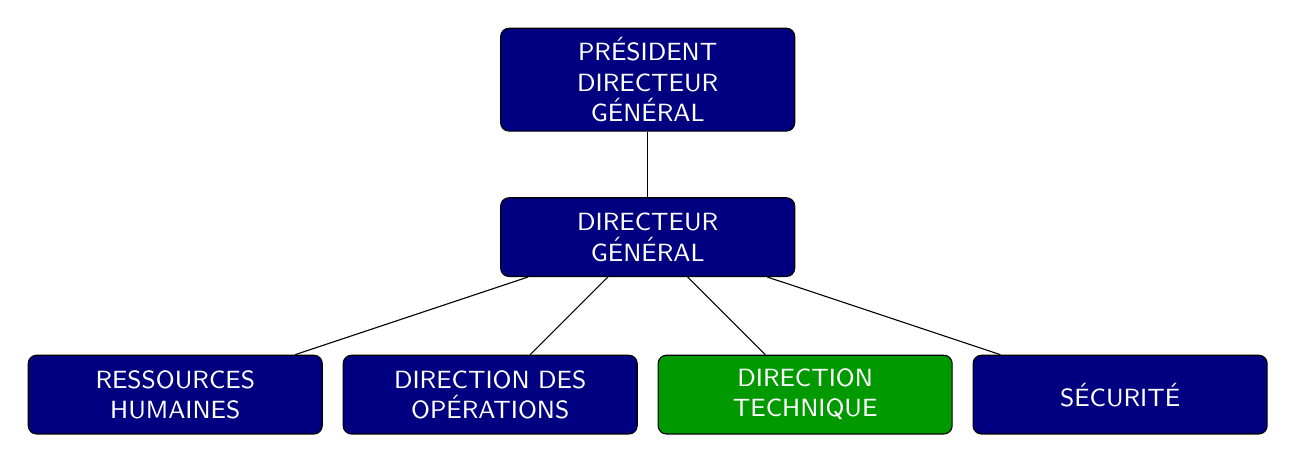
\begin{tikzpicture}[
			edge from parent/.style={draw, -},
			level 1/.style={sibling distance=60mm, level distance=20mm},
			level 2/.style={sibling distance=40mm, level distance=20mm},
			every node/.style={
					draw,
					fill=blue!50!black,
					rounded corners=3pt,
					text=white,
					align=center,
					font=\sffamily\small,
					text width=35mm,
					minimum height=10mm
				}
		]
		\node {PRÉSIDENT \\ DIRECTEUR \\ GÉNÉRAL}
		child {node {DIRECTEUR \\ GÉNÉRAL}
				child {node {RESSOURCES \\ HUMAINES}}
				child {node {DIRECTION DES \\ OPÉRATIONS}}
				child {node[
								draw,
								fill=green!60!black, % Changer la couleur ici
								rounded corners=3pt,
								text=white,
								align=center,
								font=\sffamily\small,
								text width=35mm,
								minimum height=10mm
							]{DIRECTION \\ TECHNIQUE}
					}
				child {node {SÉCURITÉ}}
			};
	\end{tikzpicture}
	\caption{Organisation interne simplifiée de l'entreprise}
\end{figure}

\subsection{Produits et services de l'entreprise}

Oneex propose une gamme de solutions matérielles et logicielles, parmi lesquelles trois produits phares :

\begin{itemize}
	\item \textbf{Oneex Desktop} : une station de vérification d’identité clé en main simple et intuitive pour un accueil sécurisé , cette derniere effectue chaque scan en toute confiance. Le desktop Oneex reconnaît instantanément tous les documents d'identité de 197 pays — garantissant une vérification sûre et précise à chaque fois.
	      \begin{figure} [H]
		      \centering
		      \includegraphics[width=.5\textwidth]{figures/Oneex desktop.png}
		      \caption{Oneex Desktop}
	      \end{figure}
	\item \textbf{Oneex Suitcase} : une valise mobile permettant de réaliser des contrôles sur le terrain , portable et robuste , elle laisse les utilisateurs se profiter d’un système mobile de vérification d’identité fiable et sécurisé.
	      \begin{figure} [H]
		      \centering
		      \includegraphics[width=.5\textwidth]{figures/Oneex suitcase.png}
		      \caption{Oneex Suitcase}
	      \end{figure}
	\item \textbf{Oneex Kiosk} : un kiosque en libre-service pour l’accueil et le contrôle des visiteurs. Permet Accueiller vos visiteurs sans assistance grâce à une vérification rapide et un accès direct.Une solution pensée pour vos opérations, combinant biométrie avancée et automatisation complète de l’accès visiteurs.
	      \begin{figure} [H]
		      \centering
		      \includegraphics[width=.5\textwidth]{figures/Oneex kiosk.png}
		      \caption{Oneex Kiosk}
	      \end{figure}
\end{itemize}

\begin{table}[H]
	\centering
	\renewcommand{\arraystretch}{1.2}
	\begin{tabular}{|p{3cm}|p{5cm}|p{4cm}|p{2.5cm}|}
		\hline
		\textbf{Produit} & \textbf{Description}                     & \textbf{Dimensions} & \textbf{Poids} \\ \hline
		Oneex Desktop    & Station de vérification d’identité fixe  & 465 x 365 x 175 mm  & 8 kg           \\ \hline
		Oneex Suitcase   & Valise mobile de contrôle sur le terrain & 560 x 365 x 230 mm  & 12 kg          \\ \hline
		Oneex Kiosk      & Kiosque en libre-service autonome        & 1640 x 450 x 460 mm & 65 kg          \\ \hline
	\end{tabular}
	\caption{Caractéristiques physiques principales des solutions matérielles Oneex}
\end{table}
Ces produits sont complétés par la suite logicielle Oneex Cloud et ScanApp, garantissant un pilotage centralisé et une intégration fluide dans les environnements clients.

Son application \emph{Oneex Cloud}, une plateforme offre un contrôle centralisé et un suivi avancé des vérifications d’identité.

Cette plateforme permet un :

\begin{itemize}
	\item \textbf{Suivi des documents scannés} : historique complet, résultats détaillés et traçabilité optimale.
	\item \textbf{Demande d’expertise} : sollicitation d’experts pour garantir des analyses approfondies et fiables.
	\item \textbf{Statistiques avancées} : exploitation des tendances de la fraude pour optimiser la gestion des incidents.
\end{itemize}

Ces solutions permettent aux entreprises de contrôler efficacement les accès, de réduire les fraudes et de fluidifier les processus d’intégration dans le respect des réglementations RGPD.

\subsection{Services informatiques et outils internes}

\subsubsection{Les services informatiques}

\textbf{Oneex ScanApp} constitue le cœur opérationnel de l’entreprise. Il assure l’analyse documentaire et la vérification d’identité, disponible sur postes fixes comme sur mobiles, avec une interface ergonomique et des fonctionnalités avancées.

Il est constitué par une une interface utilisateur intuitive pour les ecrans des solutions que oneex offre et un moteur d’analyse de documents qui tourne localement , et est chargé par la lecture des documents , et l'execution d'une vingtaine d'algorithmes pour s'assurer de l'authenticité du document scanné.
Il est composé de plusieurs modules , repartis entre le frontend et le backend, qui communiquent via des API sécurisées.
Le code de ces dernieres est hebergé sur un serveur gitlab interne, garantissant ainsi la sécurité et la confidentialité des données et il est repartit en 4 depots principaux , chacun dédié à un aspect spécifique de l'application.

\textbf{Oneex Cloud} complète cet écosystème en permettant :

\begin{itemize}
	\item la gestion des vérifications,
	\item le suivi historique et la traçabilité,
	\item la sollicitation d’experts en cas de doute,
	\item l’analyse statistique des fraudes détectées.
\end{itemize}

de meme ceci est hébergé sur un serveur gitlab interne, garantissant ainsi la sécurité et la confidentialité des données.
Ces services sont accessibles via une interface web sécurisée, permettant aux utilisateurs de gérer les opérations de vérification d’identité de manière centralisée et efficace.
L’entreprise utilise également des outils de gestion de projet et de suivi des tâches, tels que You
Track, pour assurer une coordination optimale entre les équipes et garantir la qualité des livrables.
Le système de gestion des versions est basé sur GitLab, permettant une collaboration fluide et un
suivi rigoureux des modifications apportées au code source des applications.
Le code de ces dernieres est hebergé sur un serveur gitlab interne, garantissant ainsi la sécurité et la confidentialité des données et il est representé en tant que deux parties :
* front office : qui represente l'interface utilisateur et les interactions avec les clients, incluant les applications mobiles et desktop.
* back office : qui l'interface des administrateurs et des experts, permettant la gestion des opérations, le suivi des incidents et l'analyse des données.
Chaque partie est développée en utilisant go et nuxt.js, garantissant ainsi une performance optimale et une expérience utilisateur fluide et ils sont separés en plusieurs depots, groupés en deux projets : le backend et le frontend.

\subsubsection{Les outils internes}

L’entreprise utilise plusieurs outils collaboratifs et techniques, parmi lesquels :
GitLab, Harbor, Nextcloud, Jitsi, Label Studio, YouTrack, Vault, SSO Keycloak.
Les bases de données sont hébergées sur des serveurs dédiés et sécurisés, garantissant la confidentialité et la disponibilité des informations sensibles ainsi que la conformité aux réglementations et assurer un controle et une gestion des accès rigoureux.

\subsubsection{Infrastructures internes}

Afin de garantir un contrôle total et une indépendance vis-à-vis des fournisseurs de cloud, Oneex a opté pour une infrastructure IaaS (Infrastructure as a Service) autohébergée sur des serveurs physiques administrés via la solution de virtualisation Proxmox VE.
Actuellement, l'entreprise dispose de plusieurs serveurs physiques hébergés chez Scaleway, utilisés pour héberger l’ensemble de ses VMs, systèmes critiques et clusters Kubernetes.

\begin{figure} [H]
	\centering
	\includegraphics[width=.5\textwidth]{figures/Ressources cloud.png}
	\caption{Ressources cloud de Oneex}
\end{figure}

\paragraph{Architecture réseau}

L’architecture réseau repose sur deux types de bridges configurés sur chaque hôte Proxmox :

\begin{itemize}
	\item \textbf{Bridge public (vmbr0)} : utilisé uniquement par l’hyperviseur Proxmox lui-même et le pare feu Pfsense, pour exposer certains services, . Aucune VM n’est connectée à ce bridge.
	\item \textbf{Bridge interne (vmbr1)} : représente le LAN interne de l’entreprise. Proxmox y participe activement en tant que passerelle (\texttt{gateway}) pour les machines virtuelles, leur permettant un accès vers l’extérieur ou à d’autres zones du réseau.
\end{itemize}

Les services hébergés par les VMs ne sont pas exposés directement, mais à travers un \textbf{reverse proxy NGINX}, installé sur Proxmox ou dans un conteneur dédié. Cela permet une centralisation de l’accès, un contrôle de sécurité accru et une gestion fine des flux réseau.

\begin{figure} [H]
	\centering
	\includegraphics[width=.5\textwidth]{figures/Reseau inter proxmox.png}
	\caption{Réseau interne des serveurs Proxmox}
\end{figure}

\paragraph{Communications inter-sites}

Pour les échanges entre différents machines virtuelles dans des serveurs proxmox distincts , Oneex utilise un réseau privé chiffré basé sur VPN IPsec. Ce réseau interne garantit la confidentialité, l’intégrité et la performance des communications intersites sans dépendance à un cloud public.

\begin{figure} [H]
	\centering
	\includegraphics[width=.5\textwidth]{figures/Reseau intra proxmox.png}
	\caption{Communications inter-sites}
\end{figure}
